% !TEX root = ../thesis-example.tex
%
\section{Hyperledger-based Application}
\label{sec:impr:hl}

With the interfaces needed to easily expand the system being in place, we deemed it a good next step to add another Blockchain protocol. Specifically, we chose \emph{Hyperledger}. The application was successfully expanded with all necessary components built and tested, although the front-end still has problems trying to pack this new addition and sending it to the user's browser. This issue is elaborated in section \ref{sec:issues:integration}. This chapter will focus on firstly giving a broad overview of Hyperledger in section \ref{sec:impr:hl:basics} and then following up with detailing the implemented expansion in the later sections.

\subsection{Hyperledger as a Ledger Protocol}
\label{sec:impr:hl:basics}

To explain how the Systems of \emph{Hyperledger Fabric} work and what special features they offer, it makes sense to offer a comparison to the \emph{Ethereum} Blockchain - feature by feature. \emph{Hyperledger} wants to set itself apart by being a business-oriented information transfer protocol (hence, a shared ledger). Values, like tokens (e.g., \emph{Bitcoin, Ethereum}), are not a fundamental part of it.

\textbf{Authorization} \\[0.2em]
If configured, a Hyperledger Network will be split into groups, called organisations. Each organisation has a (potentially distinct) \emph{Certificate Authority (CA)}, through which membership in an organization is validated for every peer and account. Therefore, if one wants to interact with the network by for example invoking a smart contract, they must first be authenticated  by the CA. The CA even allows for group roles, so not every query to the network is accessible to everyone. These group roles were not further regarded in this task, however.

\textbf{Block Sealing} \\[0.2em]
Block sealing, the process of adding blocks to the Blockchain and therefore changing it's active state and log, is an essential part of Blockchain technology. In more known protocols like \emph{Bitcoin} or (at least at the time of writing) \emph{Ethereum}, the content of the next block is decided by the node that first managed to solve a cryptographic puzzle - the solving of this puzzle being called \emph{mining}. This, however, means that the time of sealing a block is somewhat random - and a bidding process is necessary to convince the block sealer of writing one's data. \newline
Hyperledger circumvents this competition-based method and instead introduces an \emph{orderer} node, which generally tries to apply block-additions in a first-in-first-out fashion (and accounts for concurrency issues). This means a more reliable way of querying the blockchain, since all actions are executed as fast as resources allow, and also because competing peers are treated equally instead of based on their bid. \newline
Additionally, from a security standpoint, a network can not as easily be 'poisoned' (by holding such a large amount of tokens or mining power that the holder can essentially decide which transactions to incorporate), since the finances and mining capacities of peers are disregarded completely.

\begin{figure}[h]
	\centering
	\captionsetup{justification=centering,margin=2cm}
	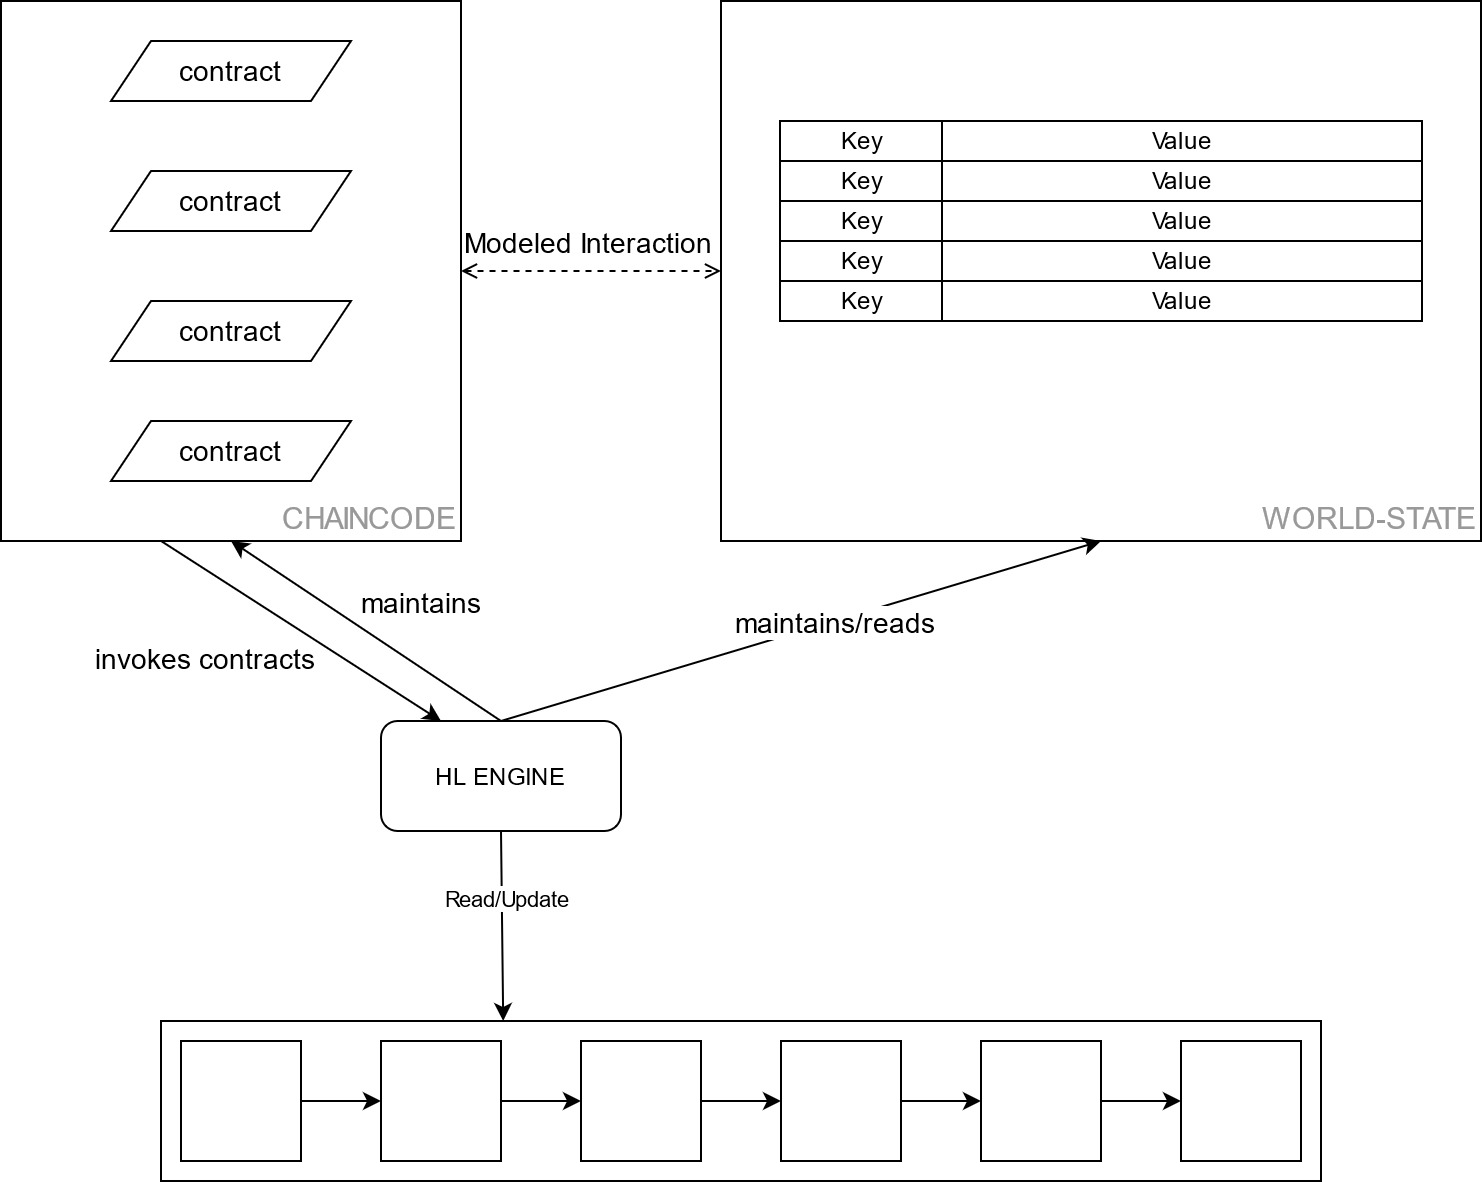
\includegraphics[height=0.7\textwidth]{gfx/hl-abstraction}
	\caption{Sketch of \emph{Hyperledger's} abstraction mechanism.}
	\label{fig:impr:hl:basics:abstraction}
\end{figure}

\textbf{Abstraction: \emph{World State \& Chaincode}} \\[0.2em]
As depicted in figure \ref{fig:impr:hl:basics:abstraction} by an 'engine' component (although this is a big simplification), Hyperledger has functions in place to display the underlying Blockchain's contents in a more abstract way, so that the user or developer doesn't need to bother with physical addresses, but may instead find them in a more human-readable format. \newline
The \emph{World State} Container is a synchronous representation of all data present in Hyperledger's underlying Blockchain, meaning that the data points present are always a representation their most recent update. Additionally, the World State is arranged like a dictionary, so that every structure inside is reachable by a key, defined by the user itself. This way, the programmer doesn't have to worry about physical addresses of the data. \newline
In the \emph{Chaincode} containers one can find the Smart Contract objects one would also find in other Blockchain application. However, these contracts are not stateful and therefore do not contain any data besides the location of the World State, where the data may be contained. In comparison, an \emph{Ethereum}-based contract may have private data and would therefore be stateful. Additionally, Chaincodes are also invocable via name, specifically by a combination of the parent contract name and the function that is to be executed.

\subsection{Component Overview}
\label{sec:impr:hl:requirements}

\begin{figure}[h]
	\centering
	\captionsetup{justification=centering,margin=2cm}
	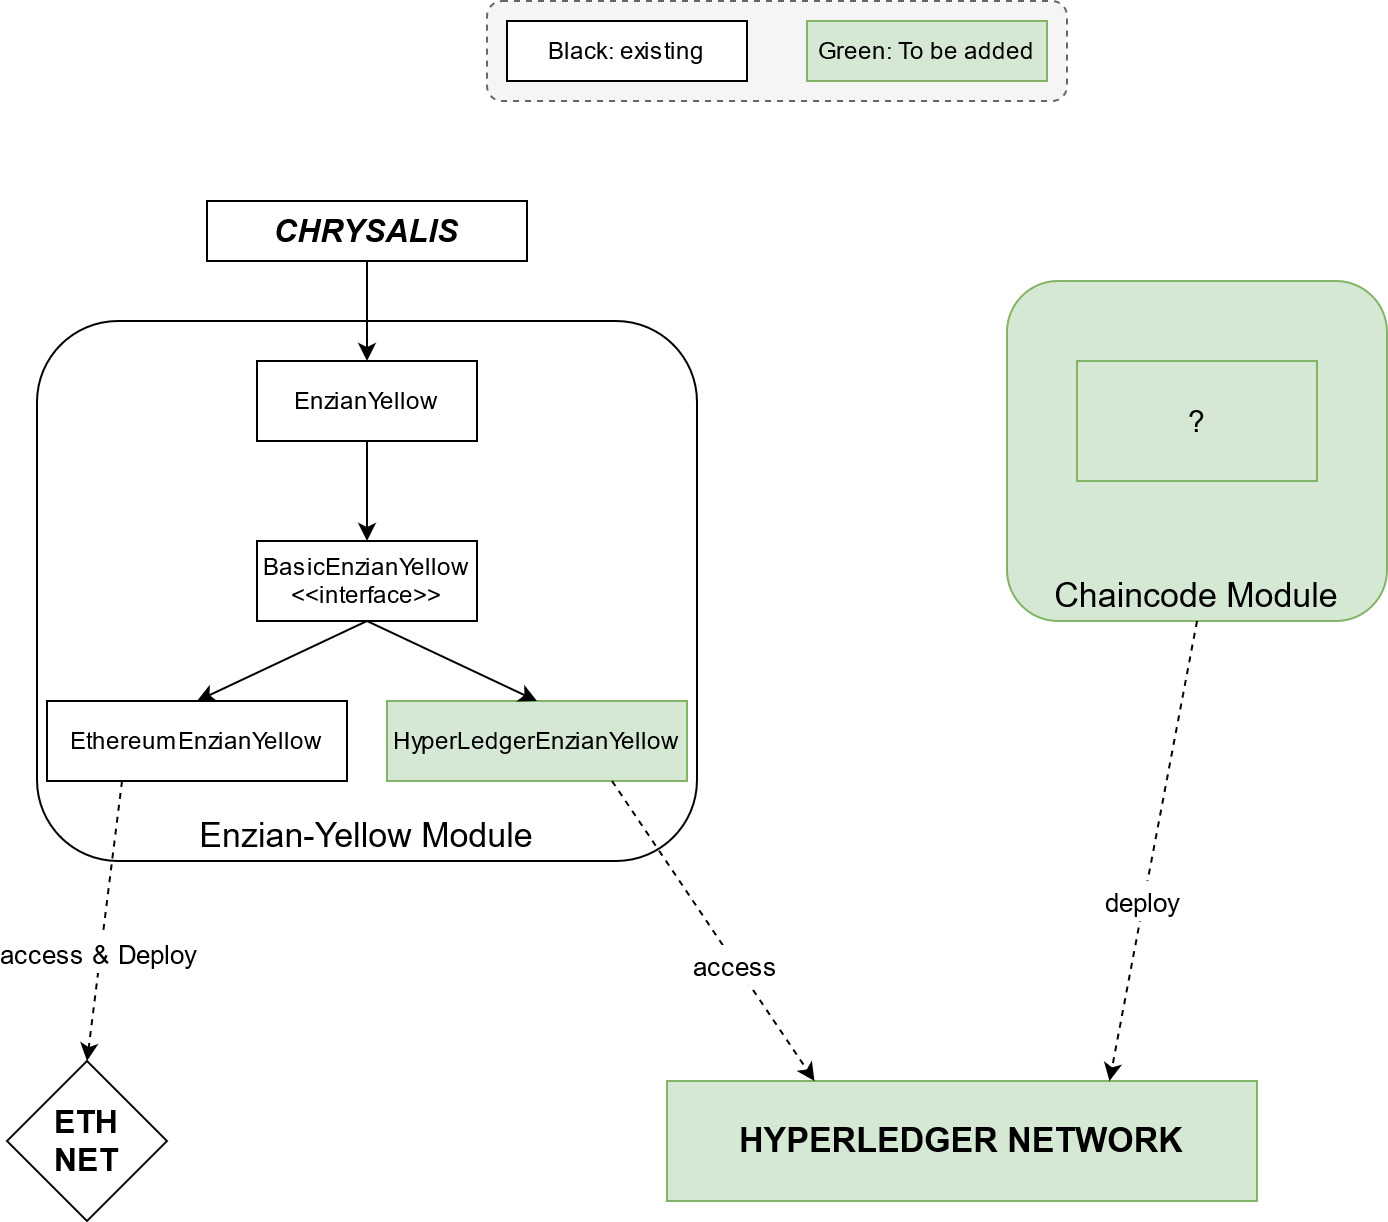
\includegraphics[width=\textwidth]{gfx/hl-structure}
	\caption{Planned and implemented module structure after adding the \emph{Hyperledger} protocol}
	\label{fig:impr:hl:structure}
\end{figure}

Three components will be needed to build a running Hyperledger-based application for the Chrysalis project. \newline
First of all, a Hyperledger Network must be established in the first place, so all necessary structures can be deployed there. Secondly, being the most complex component of the three, the Chaincode must be defined along with the data structures it uses. This module may be written and deployed in generic JavaScript thanks to Hyperledger's flexibility regarding the deployed language (e.g., this module could also be written in \emph{Go}). As per Hyperledger's requirements, the module must be contained in a separate package that can locally install dependencies and can be packed into a compressed file. Once this package is deployed, an API is needed in \emph{Enzian-Yellow} to access the Network and use the deployed components. This step is fairly straightforward, since Hyperledger Fabric provides this API and the structure of the \emph{HyperledgerEnzianYellow} can mostly be mirrored from that of \emph{EthereumEnzianYellow}.

\subsection{Test-Network}
\label{sec:impr:hl:network}

To keep development effort low, the Hyperledger Network where the contracts and data may be deployed was not built from scratch, but instead the "test-network" from Hyperledger's \emph{fabric-samples} repository was used. This network came with the features stated below.

\textbf{Network Deployment:} Instead of having to configure every network node, having to start it manually and registering it to the network, the test-network spares the developer from this work by making a running network with isolated components available as a composition of \emph{Docker}-Images. Additionally, with the help of pre-written scripts, the user may easily instantiate said composition.

\textbf{Reset functionality:} With a pre-written script, the developer may also simply wipe the entire network and bring it down. This makes development especially easy, since no trace (potentially even illegal states) of previous work will be left on the Blockchain.

\emph{Multi-Organization Scenario:} If instantiated with the right parameters, the network would come up with two organizations created, both containing one network peer each and reporting to a certificate authority. This configuration is useful, since the developer can make sure their application would run in a realistic scenario where their application and contracts must be validated by all network-registered organizations. The test-network also offers a lot of helpful scripts to make interactions with it a bit less cumbersome, e.g., so that Chaincodes may be deployed with less steps.

\subsection{Representation of Processes}
\label{sec:impr:hl:datastructure}

TODO first model the objects in the world state and how to read/save them

\begin{figure}[h]
	\centering
	\captionsetup{justification=centering,margin=2cm}
	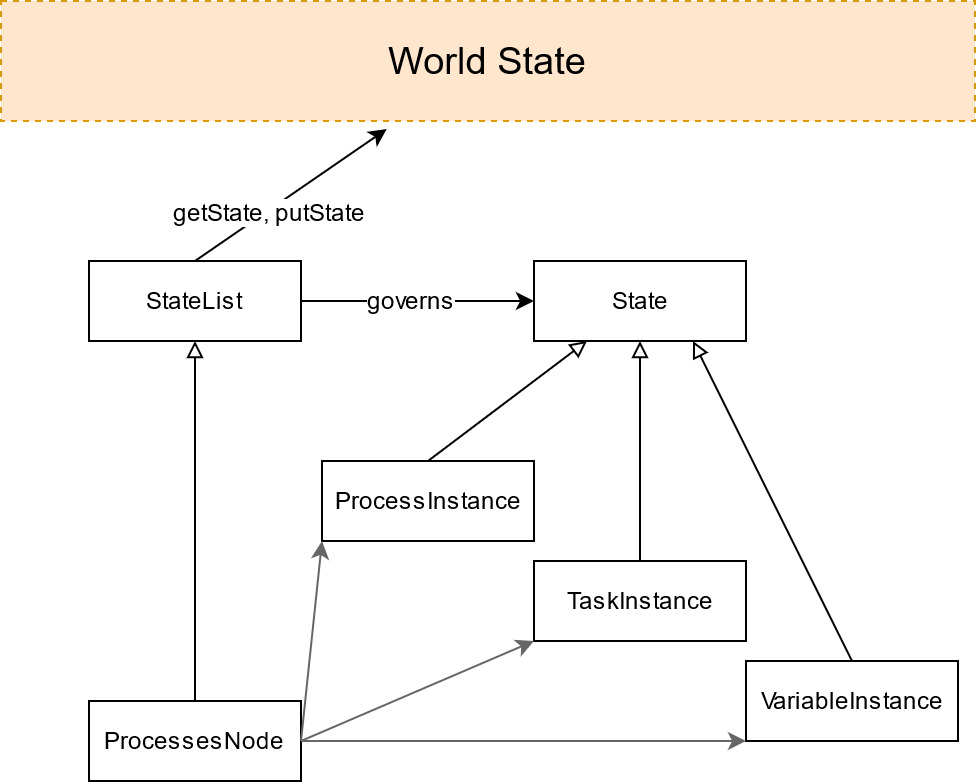
\includegraphics[width=0.8\textwidth]{gfx/hl-data}
	\caption{Data Structure deployed on the World State (State) as well as the objects that actively read and write on it (StateList)}
	\label{fig:impr:hl:data}
\end{figure}

TODO then implement Process representations on that

\subsection{Process Deployment and Execution}
\label{sec:impr:hl:chaincode}

\begin{figure}[h]
	\centering
	\captionsetup{justification=centering,margin=2cm}
	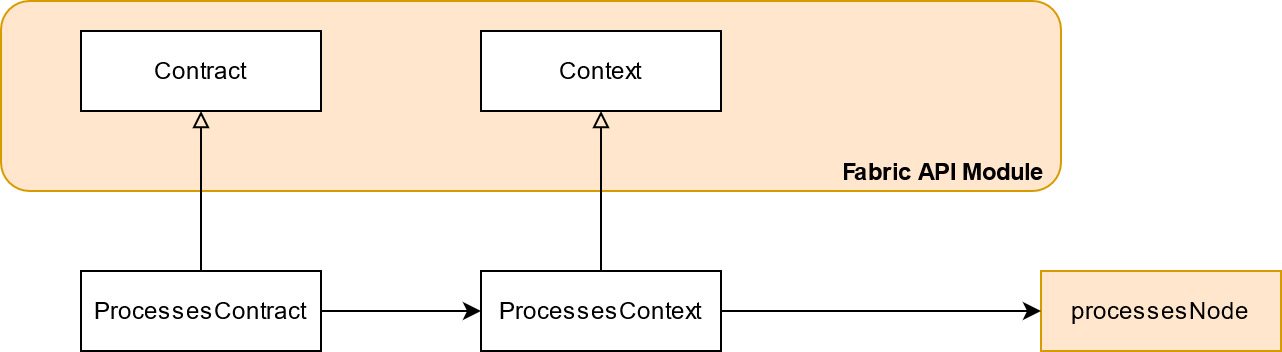
\includegraphics[width=\textwidth]{gfx/hl-contract}
	\caption{Structure of a Chaincode (Contract) together with it's gateway object that points to the World State (Context)}
	\label{fig:impr:hl:contract}
\end{figure}

\subsection{Integration into Chrysalis}
\label{sec:impr:hl:integration}

TODO explain API a bit, otherwise as in pres

\subsection{Result}
\label{sec:impr:hl:result}

TODO mention issue